\documentclass[border=10pt]{standalone}
% Shared style for the EMONI diagrams. Build: tectonic <file>.tex, then pdftocairo -svg.
\usepackage{fontspec}
\setmainfont{FiraSans}[Extension=.otf,UprightFont=*-Regular,BoldFont=*-SemiBold,ItalicFont=*-Italic,BoldItalicFont=*-SemiBoldItalic]
\setmonofont{FiraMono}[Extension=.otf,UprightFont=*-Regular,BoldFont=*-Medium,Scale=0.9]
\usepackage{tikz}
\usetikzlibrary{arrows.meta,positioning,shapes.geometric,shapes.misc,calc,fit,backgrounds}
\definecolor{eg}{HTML}{11903B}   % EMONI green
\definecolor{egl}{HTML}{E8F7EE}
\definecolor{eb}{HTML}{2A78D6}   % blue
\definecolor{ebl}{HTML}{EAF2FC}
\definecolor{eo}{HTML}{D9631E}   % orange
\definecolor{eol}{HTML}{FDF0E7}
\definecolor{ep}{HTML}{7C4DCC}   % purple
\definecolor{epl}{HTML}{F2ECFB}
\definecolor{er}{HTML}{C5221F}   % red
\definecolor{erl}{HTML}{FCEAEA}
\definecolor{ink}{HTML}{1F2328}
\definecolor{mute}{HTML}{59636E}
\definecolor{line}{HTML}{D0D7DE}
\tikzset{
  every node/.style={text=ink,font=\small},
  >={Stealth[length=2.4mm]},
  % sequence diagrams
  life/.style={draw=line,dashed,thick},
  head/.style={draw=#1,fill=#1!8,rounded corners=3pt,minimum width=27mm,minimum height=11mm,align=center,font=\small\bfseries,thick},
  act/.style={draw=#1,fill=#1!18,minimum width=2.2mm},
  msg/.style={->,thick,draw=ink},
  ret/.style={->,dashed,draw=mute},
  mlabel/.style={font=\footnotesize,fill=white,inner sep=1.5pt,align=center},
  note/.style={draw=#1,fill=#1!8,rounded corners=2pt,font=\footnotesize,align=left,inner sep=4pt},
  frag/.style={draw=mute,rounded corners=2pt},
  fraglabel/.style={draw=mute,fill=white,font=\footnotesize\bfseries,inner sep=2.5pt,anchor=north west},
  % activity diagrams
  start/.style={circle,fill=ink,minimum size=4mm,inner sep=0},
  stop/.style={circle,draw=ink,thick,minimum size=5mm,inner sep=0,path picture={\fill[ink] (path picture bounding box.center) circle (1.4mm);}},
  step/.style={draw=#1,fill=#1!8,rounded corners=5pt,thick,minimum height=9mm,minimum width=40mm,align=center,font=\small},
  step/.default=eg,
  dec/.style={diamond,aspect=2.2,draw=ink,fill=white,thick,inner sep=1.5pt,align=center,font=\footnotesize},
  flow/.style={->,thick,draw=ink},
  guard/.style={font=\footnotesize\itshape,text=mute,fill=white,inner sep=1.5pt},
  lane/.style={draw=line,fill=#1,rounded corners=4pt},
  lanetitle/.style={font=\small\bfseries,text=mute},
}

% Activity: the dashboard server checks each new reading for an overshoot and re-baselines the device.
\begin{document}
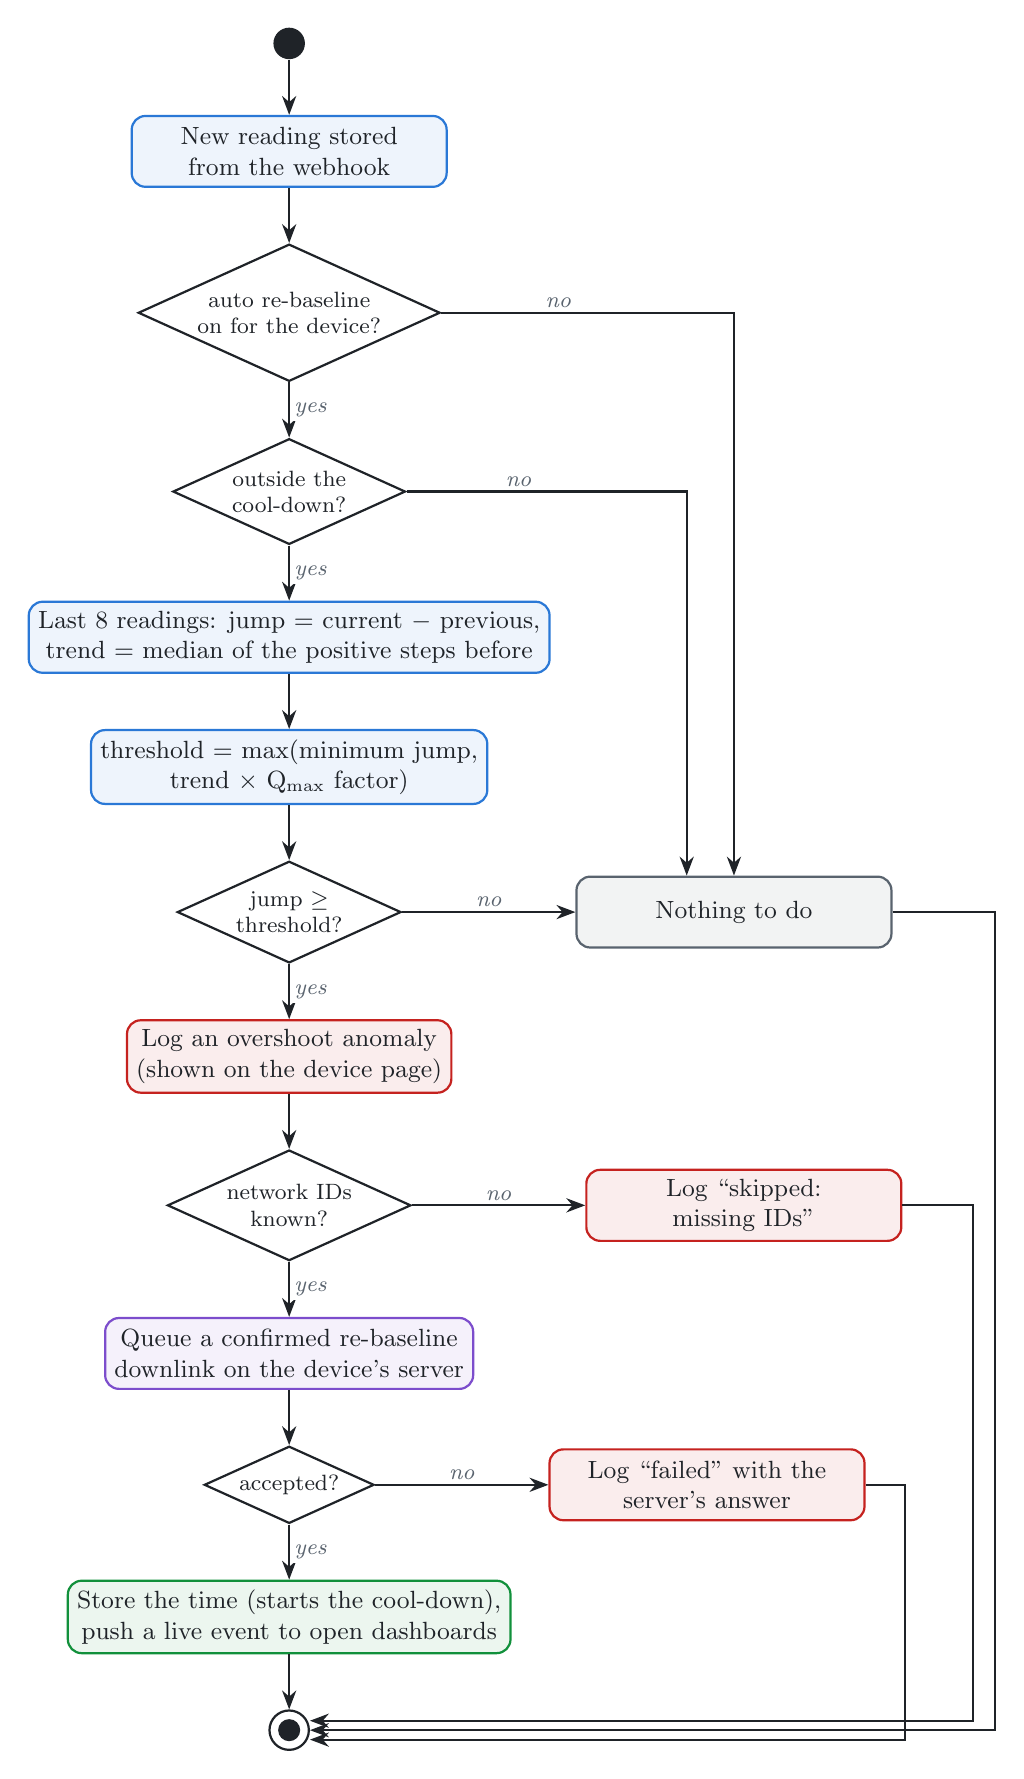
\begin{tikzpicture}[node distance=7mm and 14mm]
\node[start] (s) {};
\node[step=eb,below=of s] (in) {New reading stored\\from the webhook};
\node[dec,below=of in] (en) {auto re-baseline\\on for the device?};
\node[dec,below=of en] (cd) {outside the\\cool-down?};
\node[step=eb,below=of cd] (r) {Last 8 readings: jump = current $-$ previous,\\trend = median of the positive steps before};
\node[step=eb,below=of r] (th) {threshold = max(minimum jump,\\trend $\times$ Q\textsubscript{max} factor)};
\node[dec,below=of th] (j) {jump $\geq$\\threshold?};
\node[step=er,below=of j] (log) {Log an overshoot anomaly\\(shown on the device page)};
\node[dec,below=of log] (ids) {network IDs\\known?};
\node[step=ep,below=of ids] (dl) {Queue a confirmed re-baseline\\downlink on the device's server};
\node[dec,below=of dl] (ok) {accepted?};
\node[step,below=of ok] (done) {Store the time (starts the cool-down),\\push a live event to open dashboards};
\node[stop,below=of done] (e) {};
\node[step=mute,right=22mm of j] (skip) {Nothing to do};
\node[step=er,right=22mm of ok] (fail) {Log ``failed'' with the\\server's answer};
\node[step=er,right=22mm of ids] (miss) {Log ``skipped:\\missing IDs''};
\draw[flow] (s)--(in); \draw[flow] (in)--(en);
\draw[flow] (en)--node[guard,right]{yes}(cd); \draw[flow] (cd)--node[guard,right]{yes}(r);
\draw[flow] (r)--(th); \draw[flow] (th)--(j);
\draw[flow] (j)--node[guard,right]{yes}(log); \draw[flow] (log)--(ids);
\draw[flow] (ids)--node[guard,right]{yes}(dl); \draw[flow] (dl)--(ok);
\draw[flow] (ok)--node[guard,right]{yes}(done); \draw[flow] (done)--(e);
\draw[flow] (j)--node[guard,above]{no}(skip);
\draw[flow] (en.east)-|node[guard,above,pos=0.2]{no}(skip.north);
\draw[flow] (cd.east)-|node[guard,above,pos=0.2]{no}($(skip.north)+(-0.6,0)$);
\draw[flow] (ids)--node[guard,above]{no}(miss);
\draw[flow] (ok)--node[guard,above]{no}(fail);
\draw[flow] (skip.east) -- ++(1.3,0) |- (e.east);
\draw[flow] (miss.east) -- ++(0.9,0) |- ($(e.east)+(0,0.12)$);
\draw[flow] (fail.east) -- ++(0.5,0) |- ($(e.east)+(0,-0.12)$);
\end{tikzpicture}
\end{document}
